\chapter{Проектирование микросервисной архитектуры с помощью UML диаграмм. }

В данной главе представлено подробное описание спроектированной микросервисной архитектуры, отражающее как физическое распределение компонентов, так и их логическую взаимосвязь. Используя UML диаграммы развертывания, продемонстрировано разделение системы на микросервисы с акцентом на стандартизированные интерфейсы для обмена данными между ними, а также описаны внешние интерфейсы, обеспечивающие связь с клиентами и другими системами.

Также приведены диаграммы последовательности, иллюстрирующие все стадии маршрутизации запросов от клиента до сервера и обратно. Такой комплексный подход, включающий использование sidecar-компонентов для управления трафиком и интеграцию систем мониторинга, позволяет получить достоверную модель архитектуры, готовую к реализации и дальнейшему тестированию.


\section{Описание архитектуры системы с помощью диаграммы развертывания.}

На диаграмме развертывания (см. рис. \ref{pic:deployment-diagram-Istio}) система представлена с использованием Istio sidecar в каждом поде: Python-server, прокси‐сервер дополнены sidecar контейнерами, обеспечивающими перехват и маршрутизацию трафика. Такое решение упрощает контроль сетевых потоков и повышает наблюдаемость благодаря прямой интеграции с fluentbit, который собирает логи и метрики. Вариант без Istio (см. рис. \ref{pic:deployment-diagram-NOIstio}) показывает, как сервисы могут взаимодействовать напрямую, сохраняя более простую структуру развертывания, но при этом теряя автоматизированные возможности балансировки и политики безопасности. На обоих вариантах диаграммы отражено, что каждая виртуальная машина в кластере k3s содержит отдельные поды: один с основным приложением и sidecar (или без него), и дополнительный pod с fluentbit. Helm-чарт используется для автоматизации развертывания, что позволяет централизованно управлять конфигурациями. 

\begin{figure}[htbp]
  \centering
  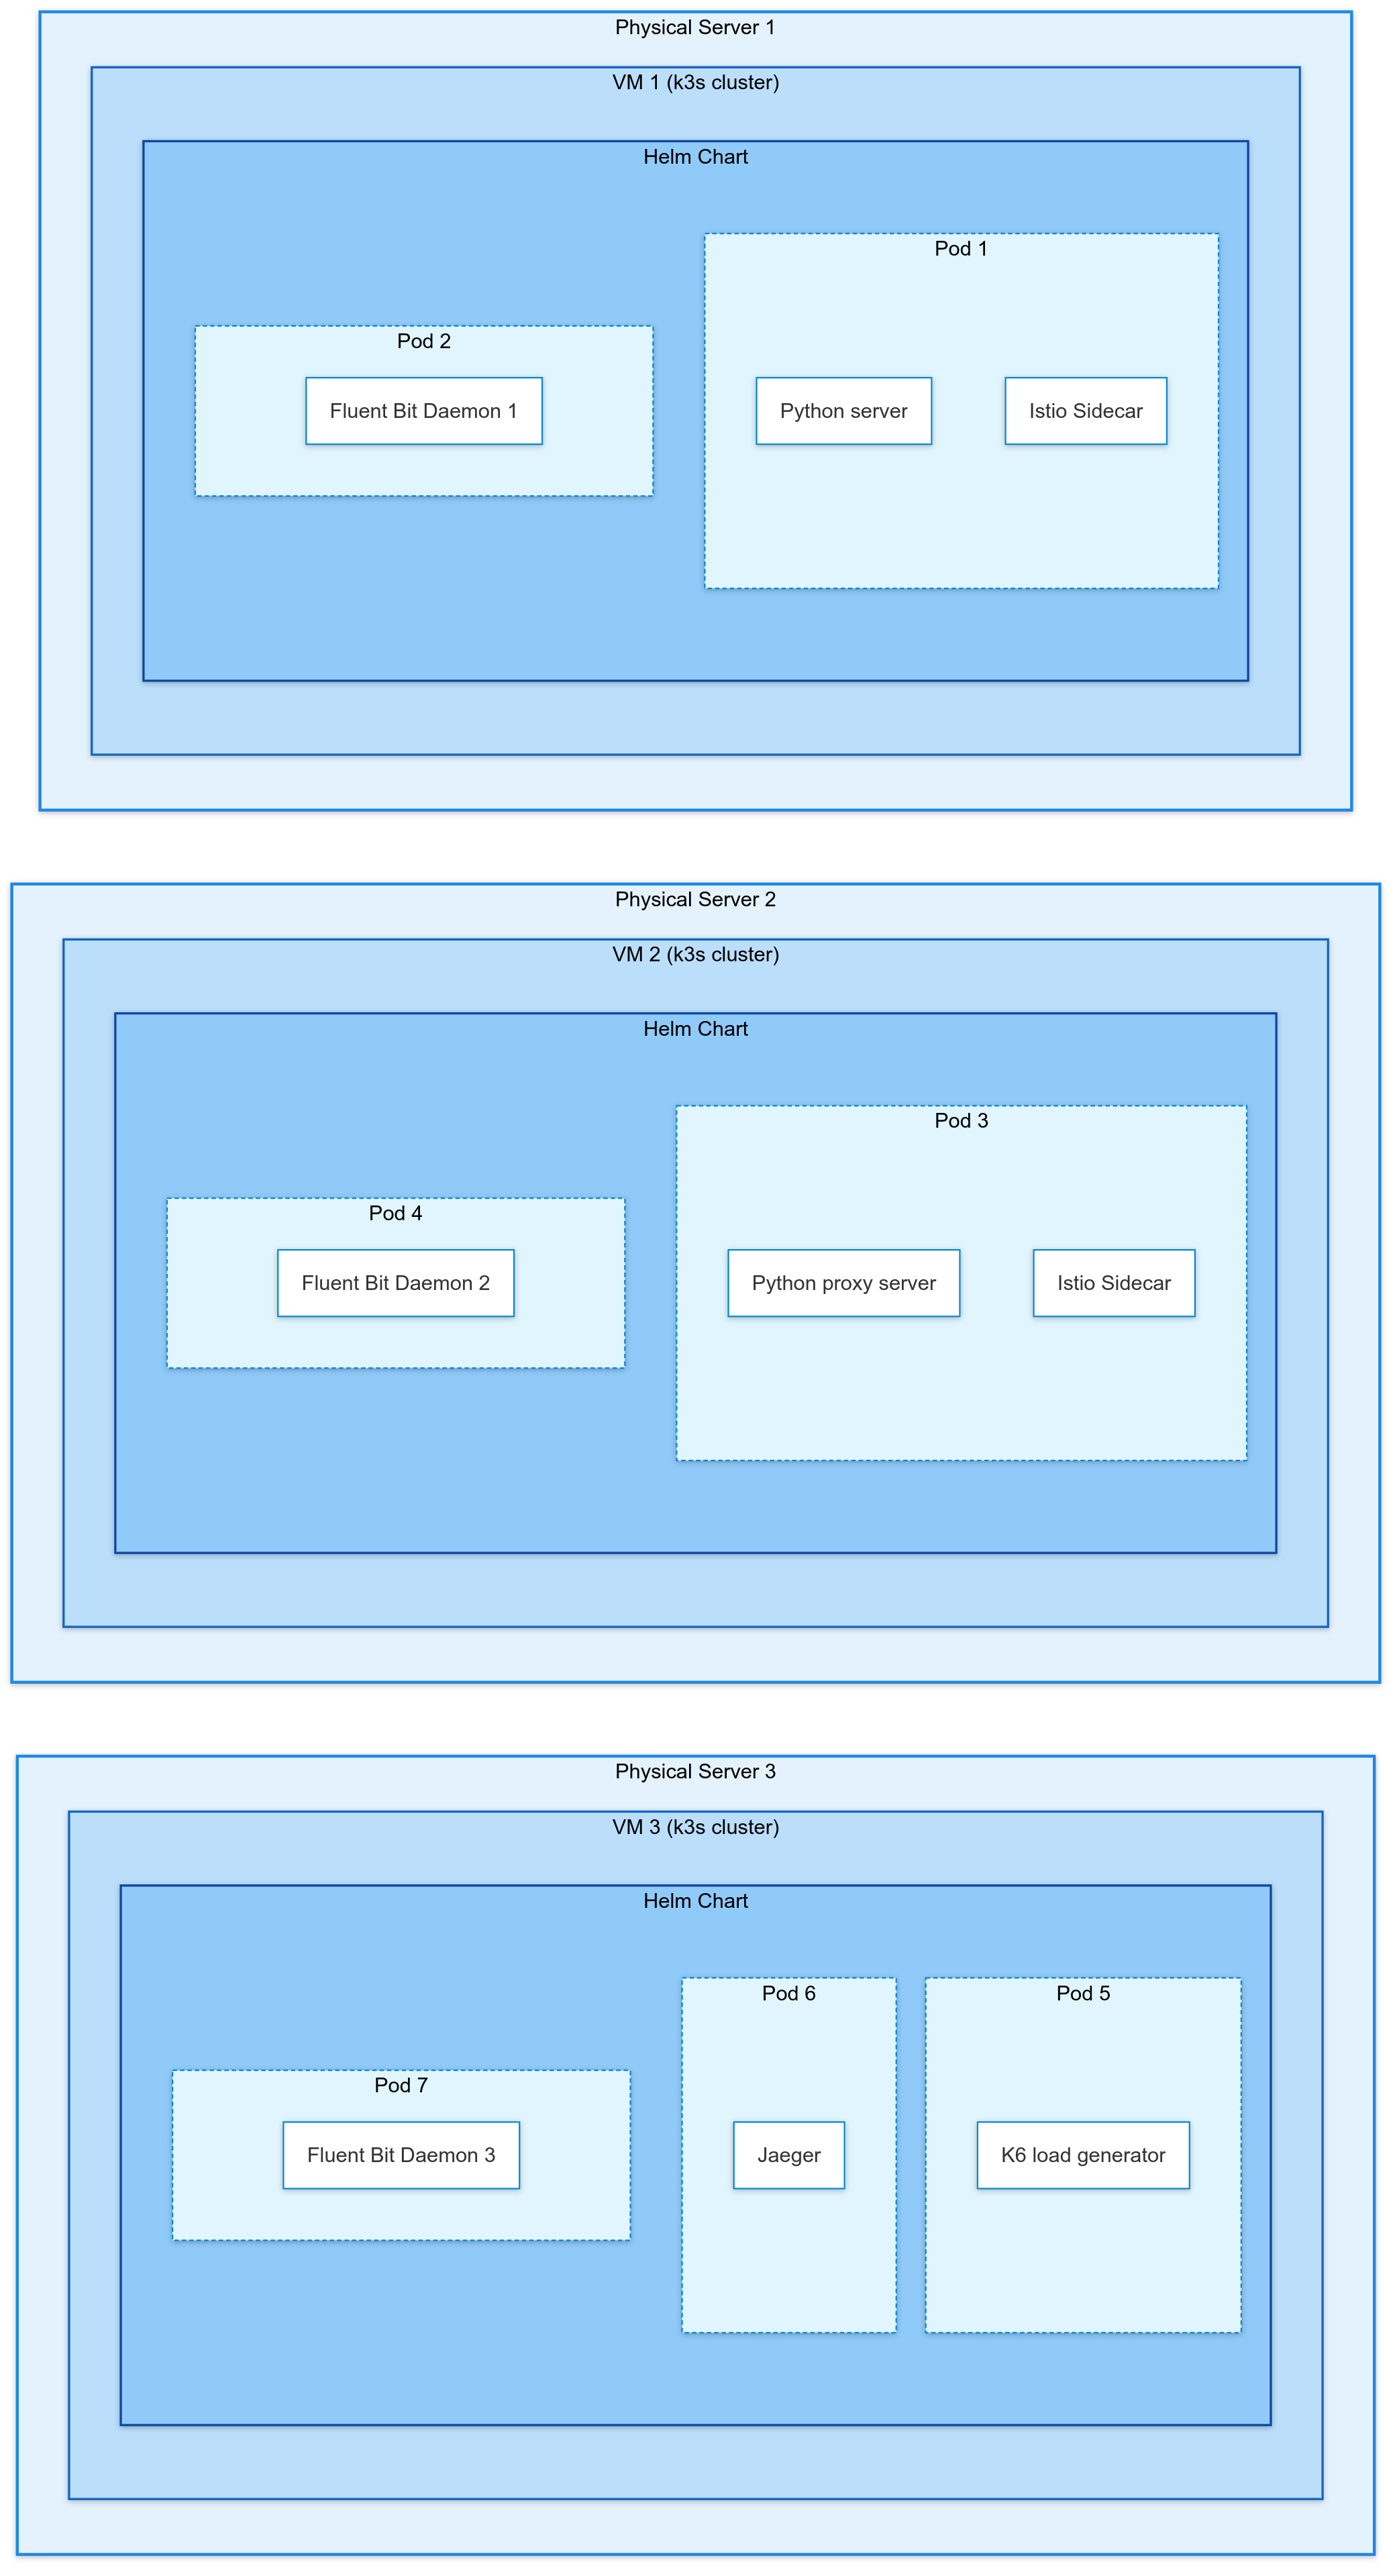
\includegraphics[
      width=\linewidth,         
      height=0.8\textheight,    
      keepaspectratio              % obey aspect ratio
  ]{img/deploy_istio.png}
  \caption{Диаграмма развертывания версии с Isito}
  \label{pic:deployment-diagram-Istio}
\end{figure}


\begin{figure}[htbp]
  \centering
  
  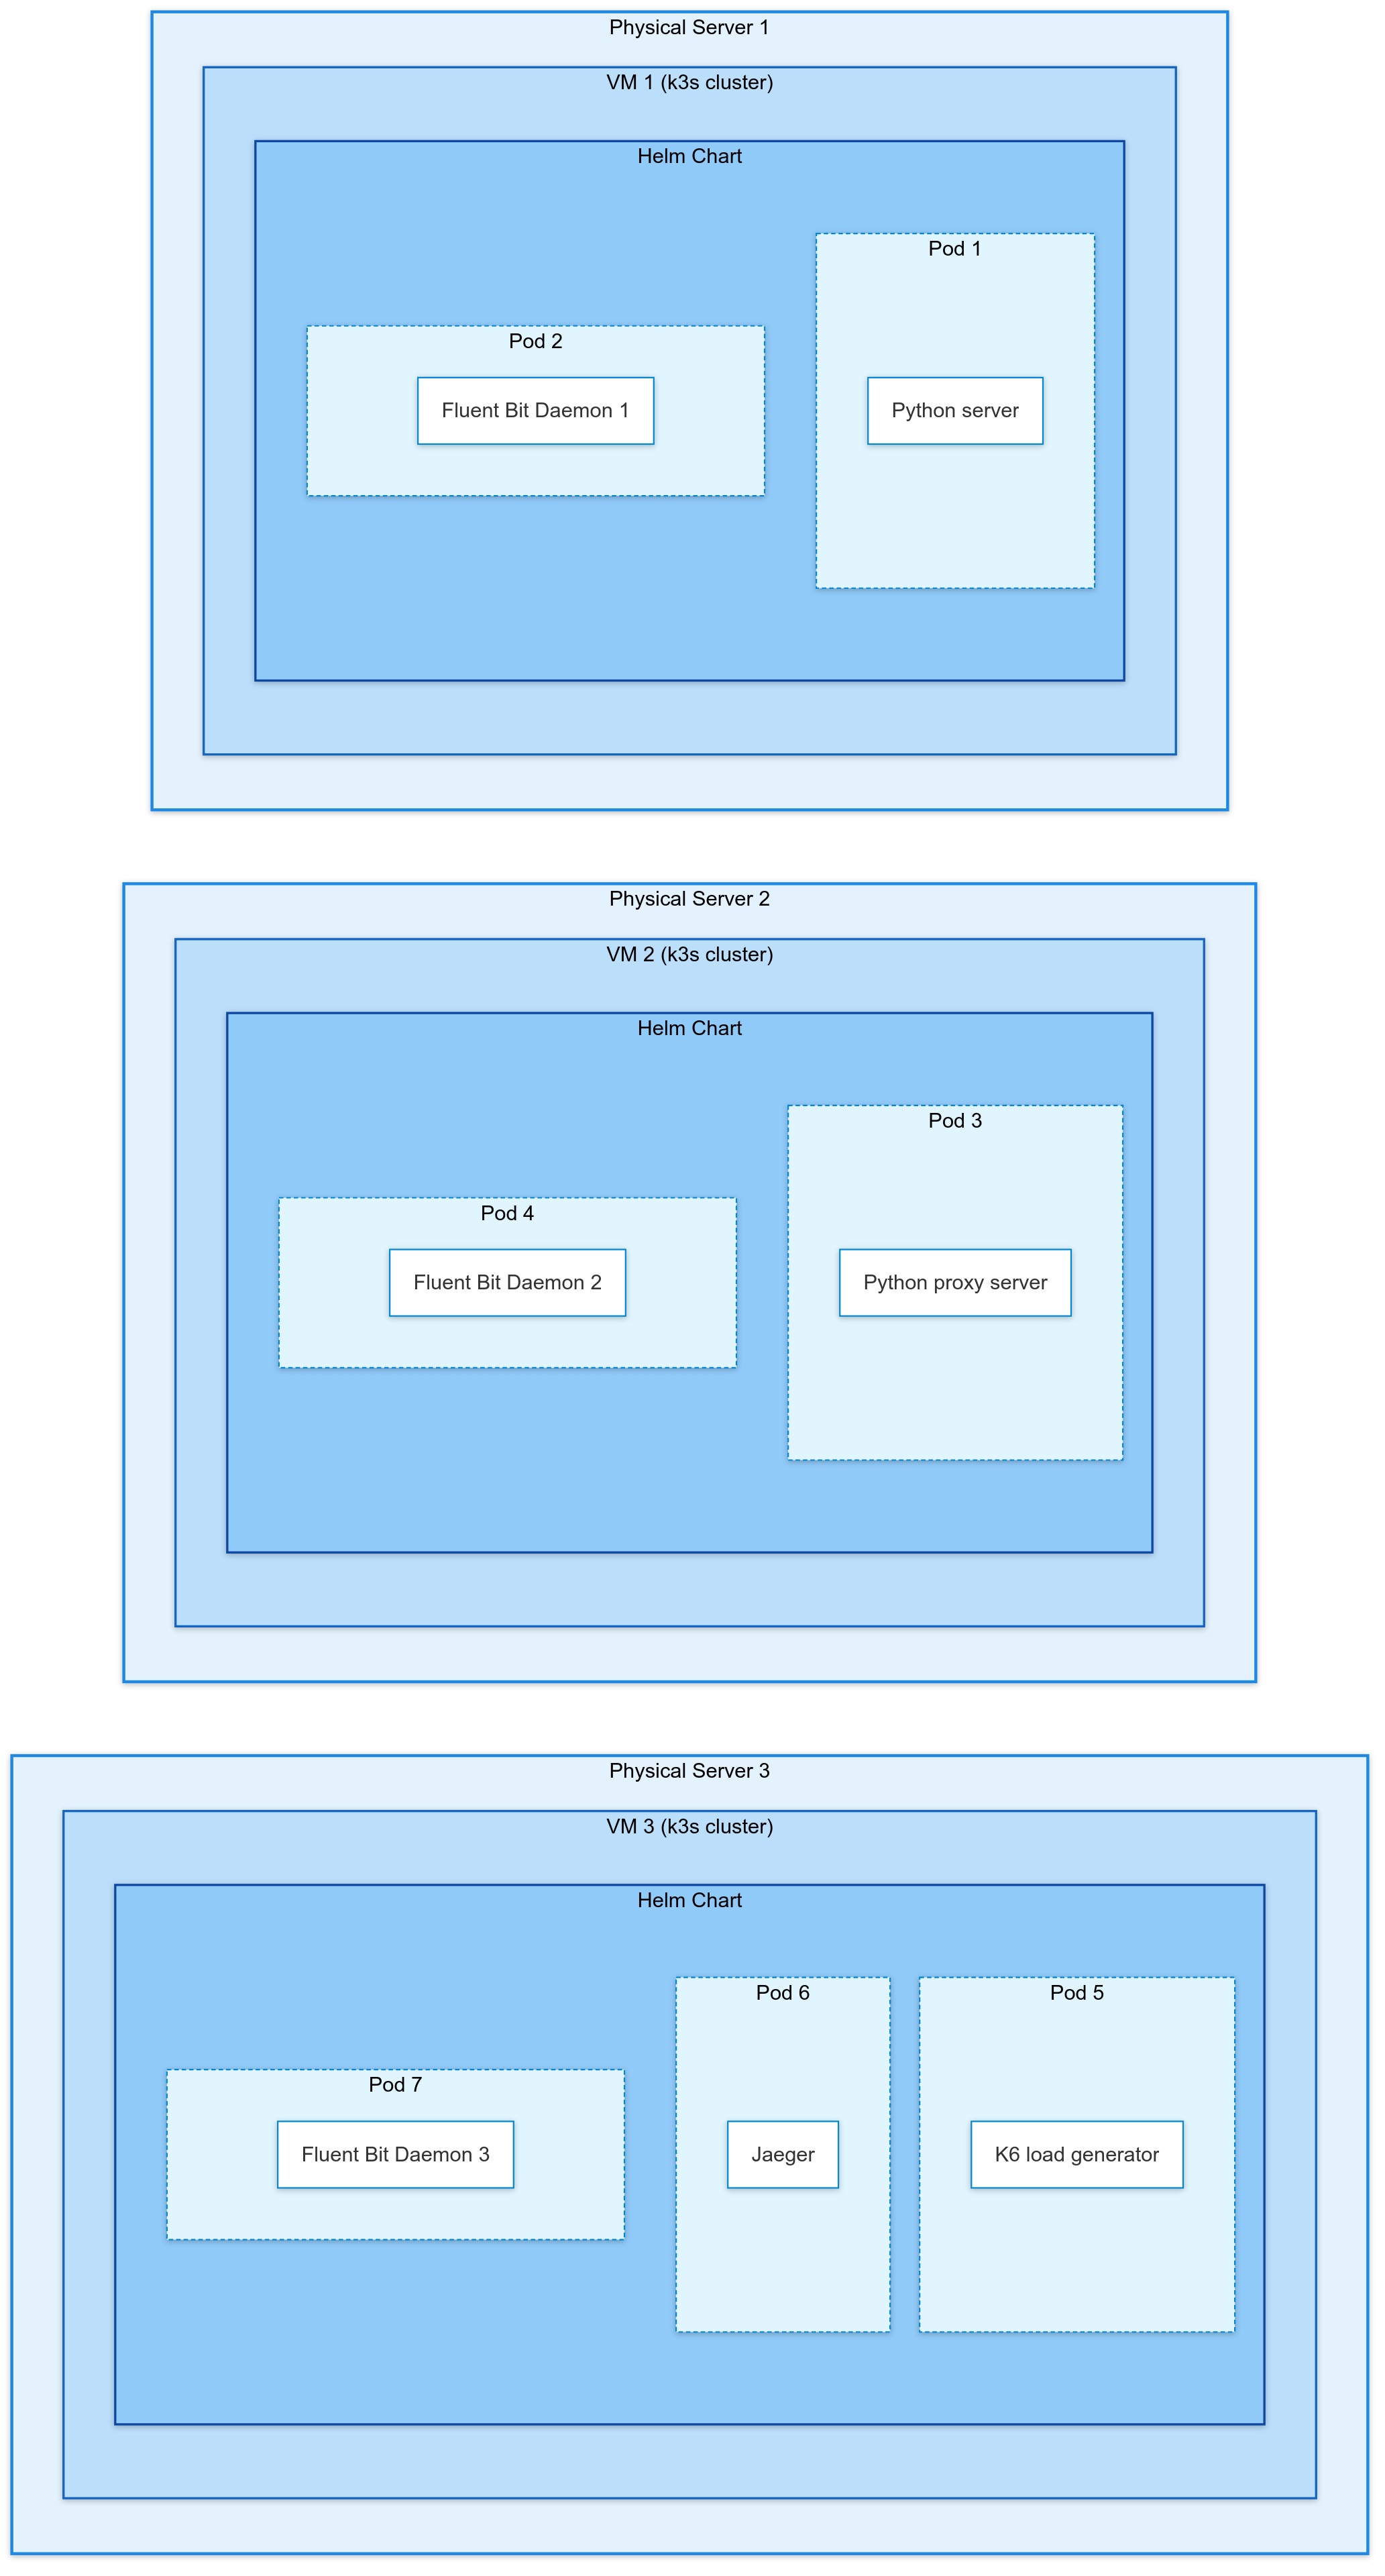
\includegraphics[
      width=\linewidth,          
      height=0.8\textheight,     
      keepaspectratio              % obey aspect ratio
  ]{img/deploy_nonistio.png}
  \caption{Диаграмма развертывания версии без Isito}
  \label{pic:deployment-diagram-NOIstio}
\end{figure}



\section{Описание архитектуры системы с помощью диаграммы последовательности.}


Диаграмма последовательности (см. рис. \ref{pic:sequence-diagram-Istio}), демонстрирует прохождение трафика через Istio sidecar: клиент формирует запрос, прокси перенаправляет его в Istio, который дополнительно проверяет доступность основного сервиса и контролирует возможные сбои. Это даёт дополнительный уровень управления и безопасности, но требует промежуточной обработки.

В варианте без service mesh (см. рис. \ref{pic:sequence-diagram-NOIstio}) реализована более простая схема обмена сообщениями: прокси общается с сервером напрямую, без дополнительного слоя Istio. Такая реализация может быть проще в настройке, но лишена встроенных возможностей мониторинга и контроля, которые предоставляет Istio.
 

\begin{figure}[htbp]
  \centering
  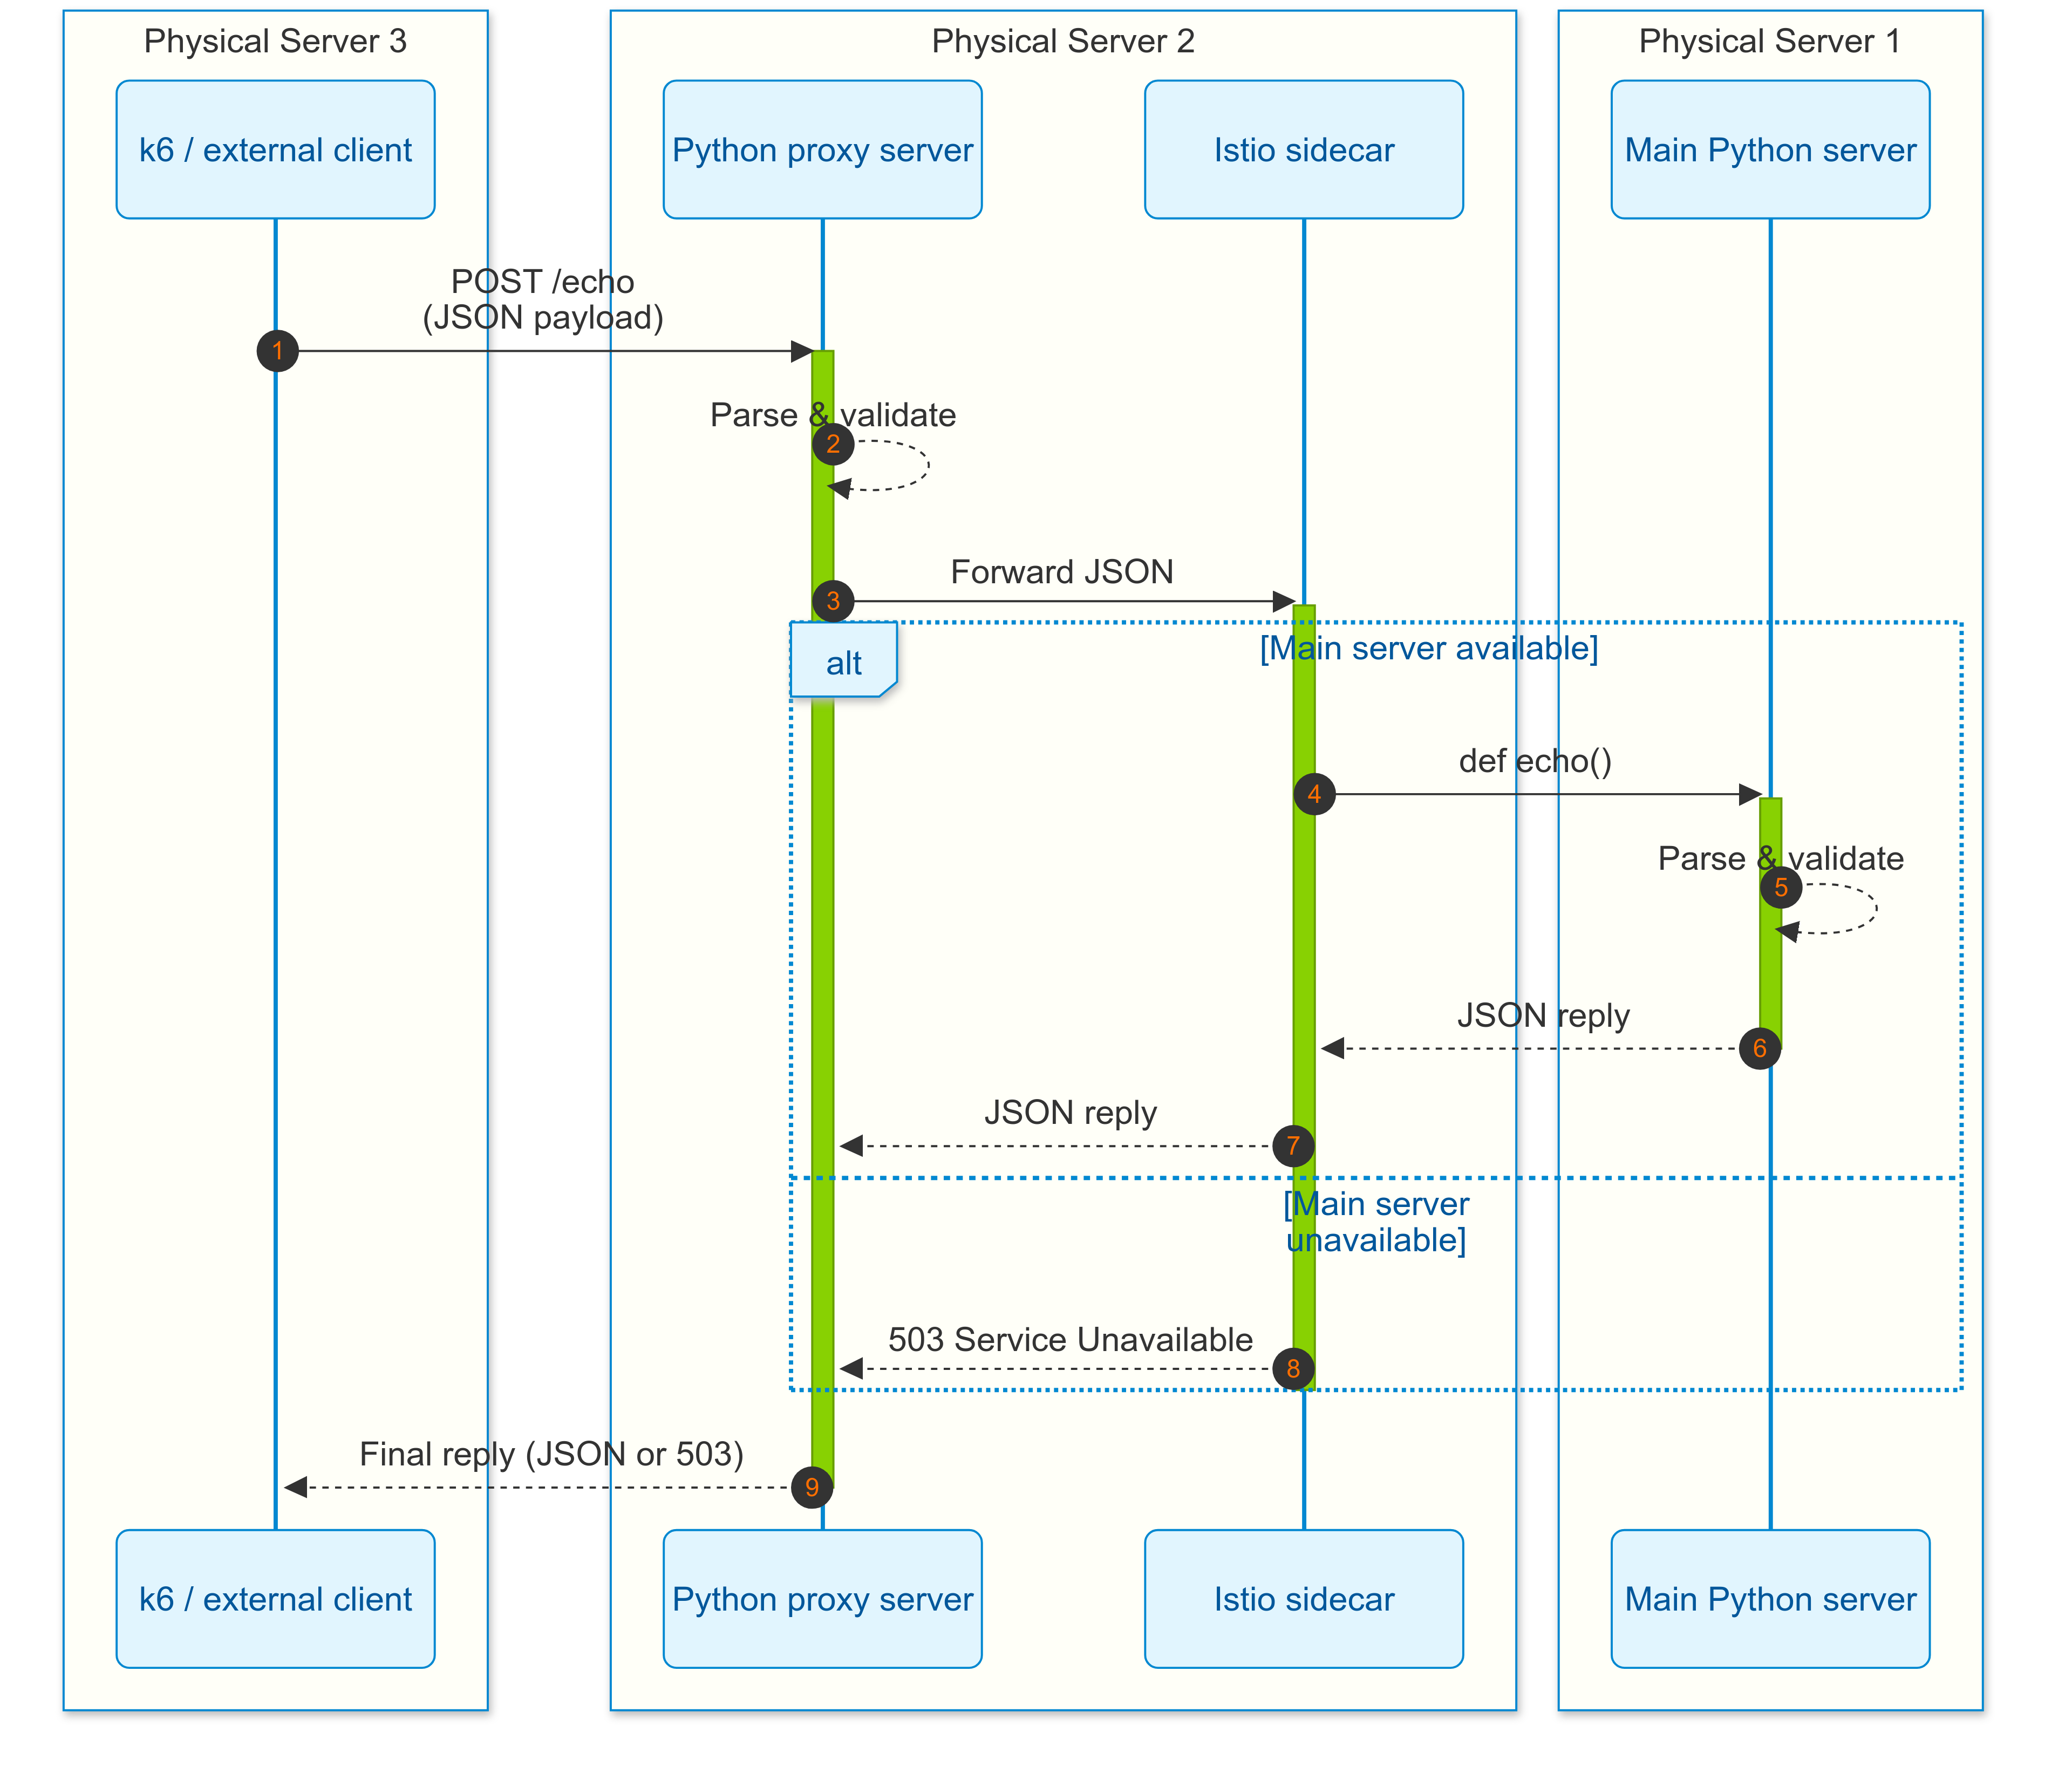
\includegraphics[
      width=\linewidth,
      height=0.8\textheight,
      keepaspectratio              % obey aspect ratio
  ]{img/seq_istio.png}
  \caption{Диаграмма последовательности версии с Istio}
  \label{pic:sequence-diagram-Istio}
\end{figure}



\begin{figure}[htbp]
  \centering
  
  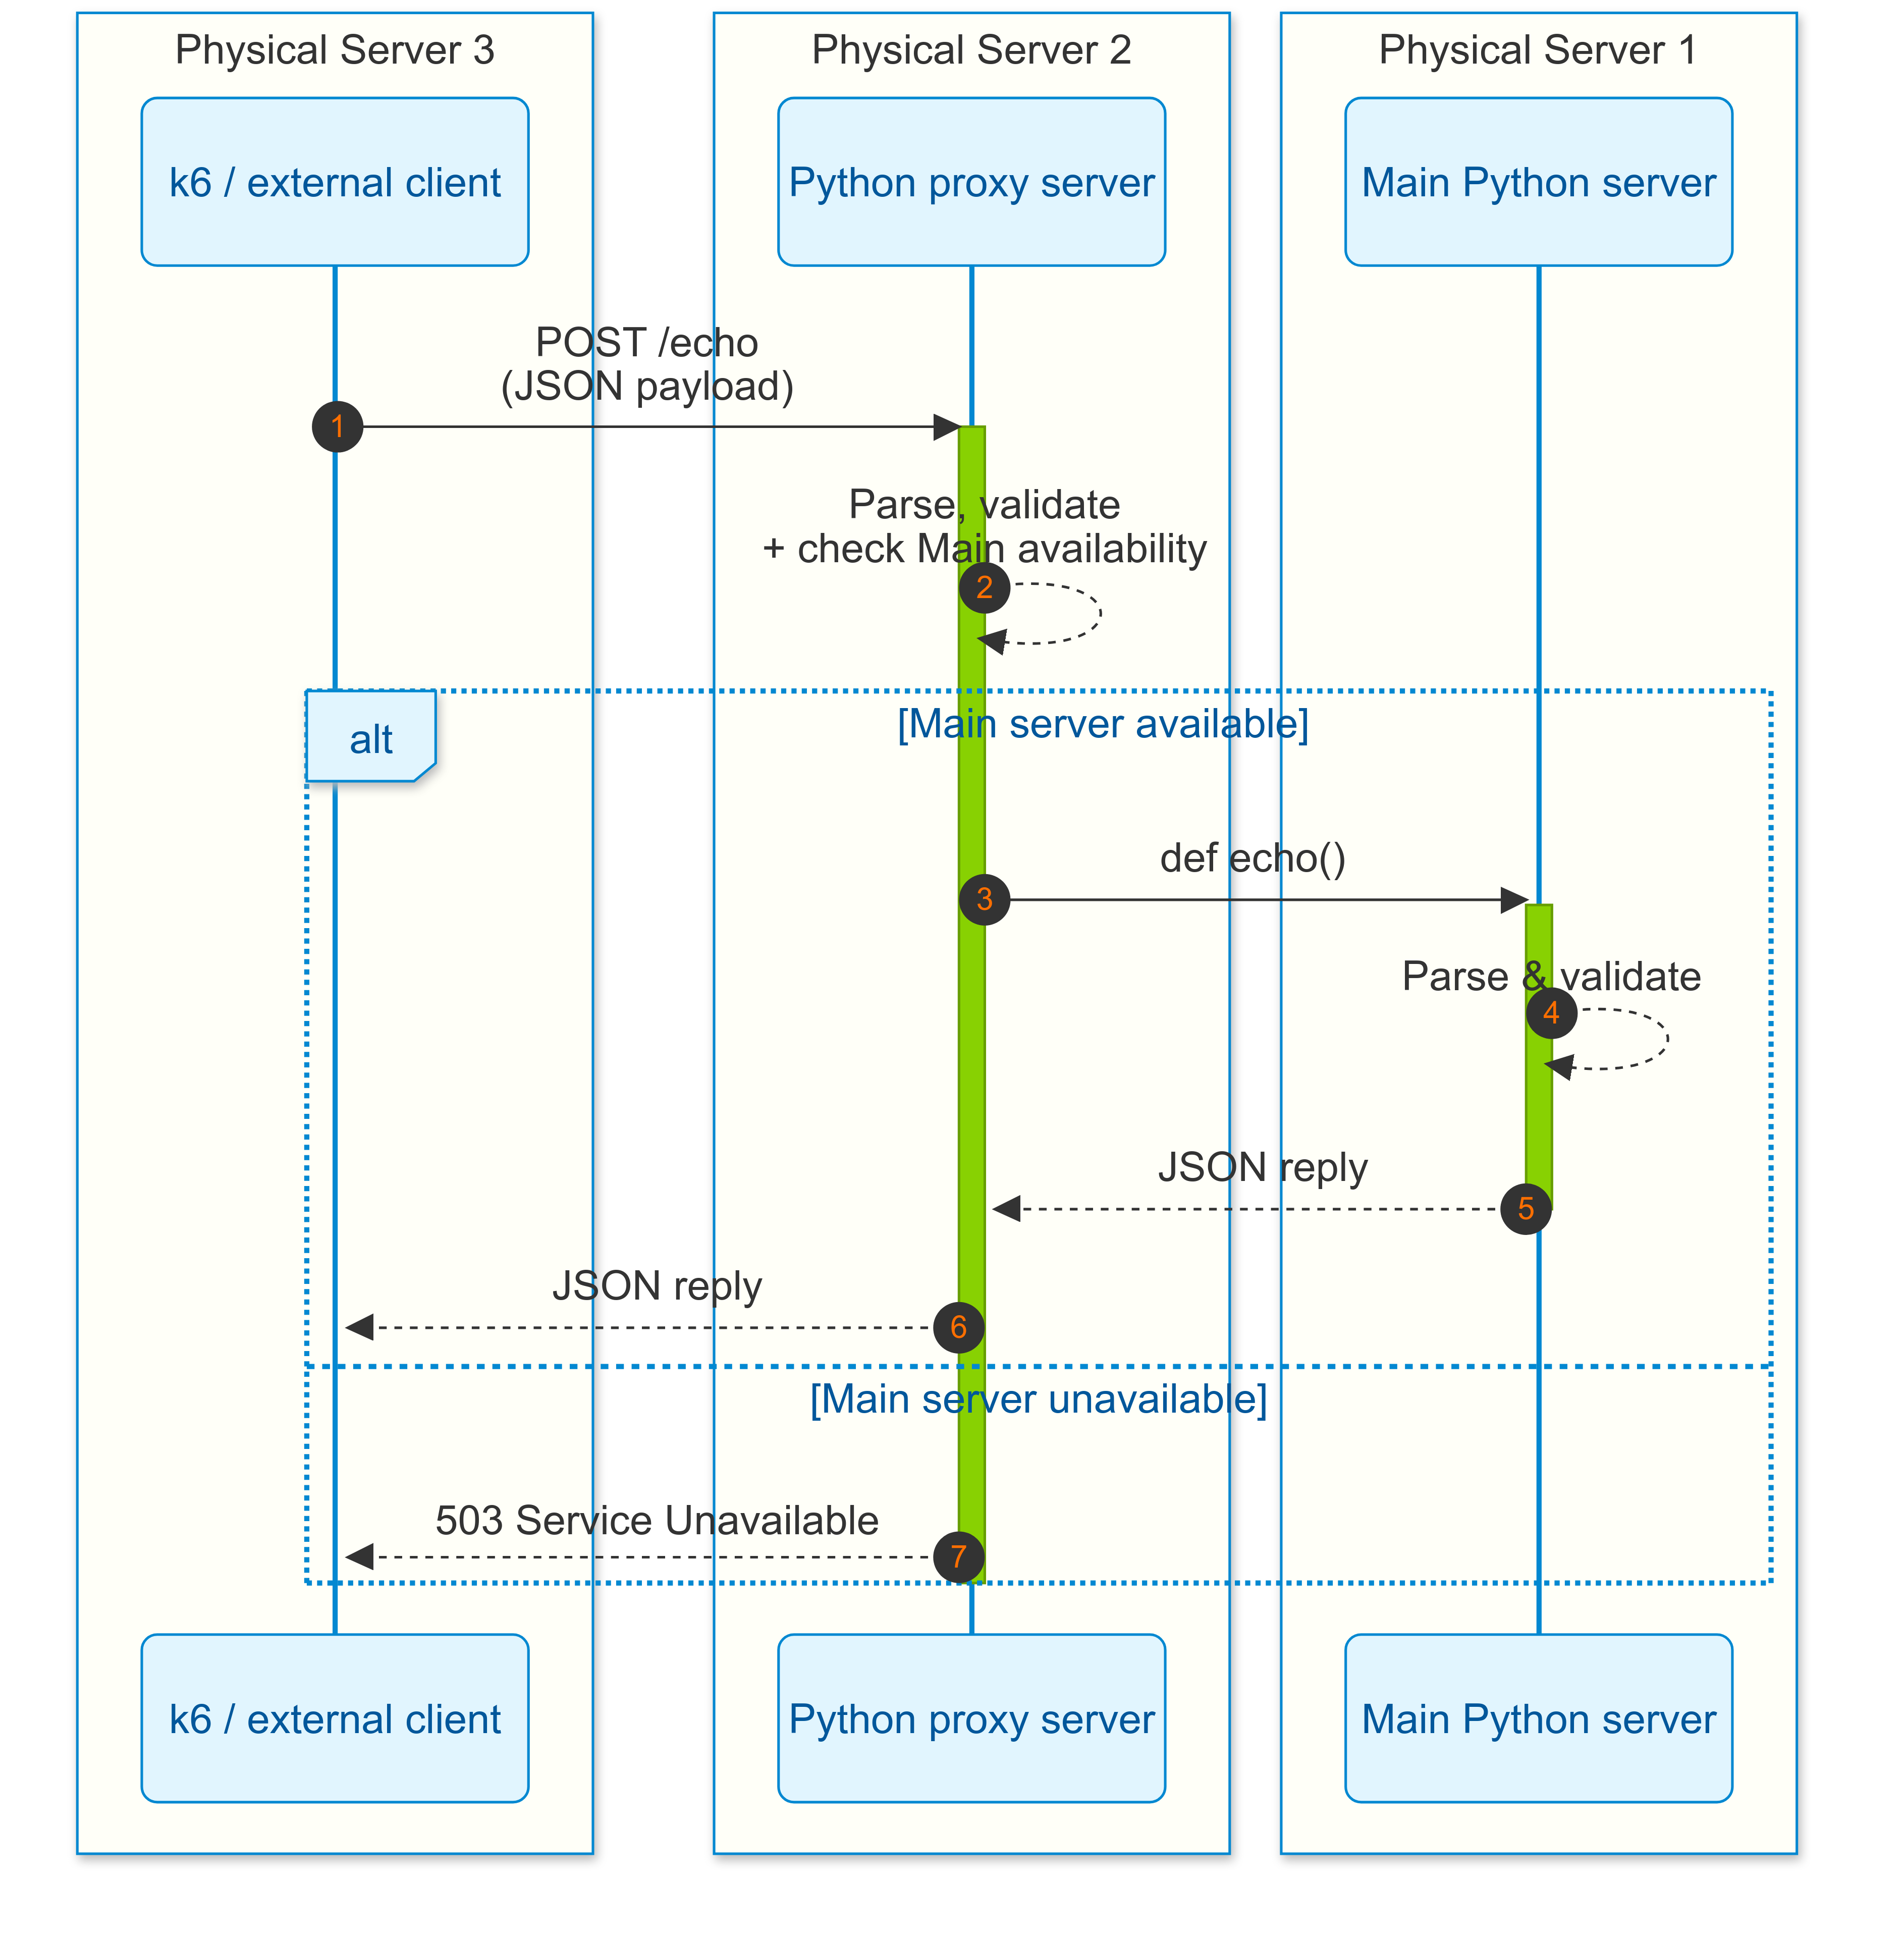
\includegraphics[
      width=\linewidth,
      height=0.8\textheight,
      keepaspectratio              % obey aspect ratio
  ]{img/seq_nonistio.png}
  \caption{Диаграмма последовательности версии без Istio}
  \label{pic:sequence-diagram-NOIstio}
\end{figure}



% Команда \texorpdfstring необходима, чтобы программа просмотра PDF документов
% верно отображала текст формул в панели оглавления.
% При отсутствии команды \texorpdfstring там, где она необходима, LaTeX выводит
% предупреждение "Token not allowed in a PDF string"


\section{Выводы}

В итоге проведённого проектирования и анализа можно заключить, что созданная модель микросервисной архитектуры учитывает все ключевые аспекты: от физической инфраструктуры и виртуальных машин в кластере k3s до логики взаимодействия сервисов в вариантах с Istio sidecar и без него. Подробно отражены потоки данных, маршрутизация и методы автоматизации развертывания, что формирует целостное представление о системе.

Разработанные диаграммы развертывания и последовательности подтвердили, что заложенные решения по управлению трафиком и сбору метрик (fluentbit, Jaeger) легко масштабируются и обеспечивают высокий уровень наблюдаемости. Таким образом, полученная модель является надёжной основой для дальнейшей реализации и проведения полноценных нагрузочных тестов.

%%% Local Variables:
%%% TeX-engine: xetex
%%% eval: (setq-local TeX-master (concat "../" (seq-find (-cut string-match ".*-3-pz\.tex$" <>) (directory-files ".."))))
%%% End:
